\documentclass[a4paper]{article}
\usepackage[spanish,es-tabla]{babel}	% trabajar en español
\spanishsignitems	
%\usepackage{simplemargins}

%\usepackage[square]{natbib}
\usepackage{amsmath}
\usepackage{amsfonts}
\usepackage{amssymb}
\usepackage{bbold}
\usepackage{graphicx}
\usepackage{blindtext}
\usepackage{hyperref}
\usepackage{amsthm}
\newtheorem{theorem}{Teorema}
\newtheorem{lemma}{Lema}
\usepackage{algorithm}
\usepackage{algorithmic}



\begin{document}
\pagenumbering{arabic}

\Large
 \begin{center}
Método de Diferencias Finitas\\


\hspace{10pt}

% Author names and affiliations
\large
%Lic. Julio A. Medina$^1$ \\
Julio A. Medina\\
\hspace{10pt}
\small  
Universidad de San Carlos\\
Escuela de Ciencias Físicas y Matemáticas\\
Maestría en Física\\
\href{mailto:julioantonio.medina@gmail.com}{julioantonio.medina@gmail.com}\\

\end{center}

\hspace{10pt}

\normalsize
\section{Ecuaciones diferenciales parciales elípticas}
La ecuación diferencial parcial elíptica a considerar es la ecuación de Poisson
\begin{equation}\label{eq::Poisson}
\nabla^2 u(x,y)\equiv \frac{\partial^2 u}{\partial x^2}(x,y) + \frac{\partial^2 u}{\partial y^2}(x,y)=f(x,y)
\end{equation}
en $R=\{ (x,y)\,\,|\,\, a<x<b ,\, c<y<d \}$, con $u(x,y)=g(x,y) \in S$, donde $S$ denota al contorno de $R$. Si $f$ y $g$ son continuas en su dominio entonces hay una única solución a la ecuación.
\subsection{Seleccionando un retículo}
El método a utilizar es una adaptación bidimensional del método de diferencias finitas para problemas con fronteras lineales como se discute en \cite{Burden}. El primer paso es escoger enteros $n$ y $m$ para definir el tamaño de los pasos(\textit{steps}) $h=(b-a)/n$ y $k=(d-c)/m$ particionando de está manera el intervalo $[a,b]$ en $n$ partes iguales de ancho $h$ y el intervalo $[c,d]$ en $m$ partes iguales con ancho $k$, formando un retículo o cuadricula como se puede ver en la figura

\begin{figure}[h]
\begin{center}
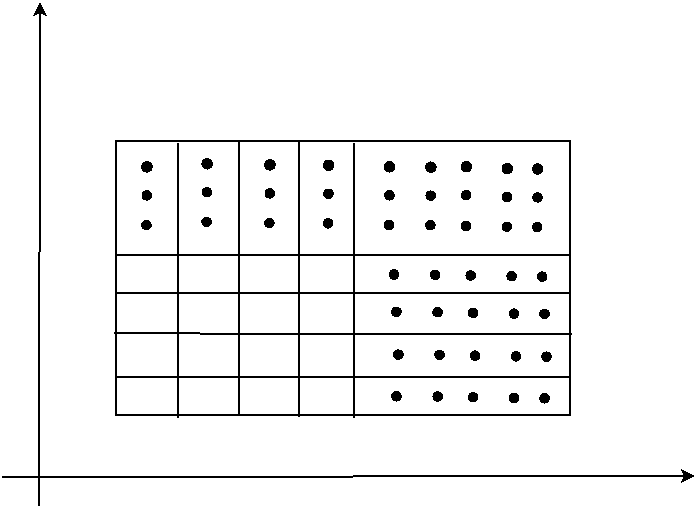
\includegraphics[scale=0.29]{./lattice.png} 
\end{center} 
\caption{Cuadricula de $n\times m$}
\label{fig::fig1}
\end{figure}
Este reticulo se construye formalmente al dibujar lineas verticales y horizontales sobre el dentro del rectagulo $R$ en los puntos con coordenadas $(x_i, y_j)$, donde
\begin{equation}
x_i=a+ih,\,\,\,\text{para cada }i=0,1,2,\hdots,n\,\,\, \text{ y } y=a+jk,\,\,\,\text{para cada }j=0,1,2,\hdots,m
\end{equation}


\section{Método de Diferencias Finitas para ecuaciones elípticas}



%En este trabajo de graduación consta de dos partes, en la primera parte se ha realizado una investigación sobre el enfoque de la mecánica estadística en la redes neuronales. En la segunda parte
\begin{thebibliography}{99}
%% La bibliografía se ordena en orden alfabético respecto al apellido del 
%% autor o autor principal
%% cada entrada tiene su formatado dependiendo si es libro, artículo,
%% tesis, contenido en la web, etc


\bibitem{Burden} Richard L. Burden, J. Douglas Faires \textit{Numerical Analysis}, (Ninth Edition). Brooks/Cole, Cengage Learning. 978-0-538-73351-9

%\bibitem{Feynman} 
%\bibitem{Hopfield} J.J. Hopfield. \textit{Neural Networks and physical systems with emergent collective computational abilities}. \url{https://doi.org/10.1073/pnas.79.8.2554}


%\bibitem{McCulloch} Warren S. McChulloch, Walter H. Pitts. \textit{A LOGICAL CALCULUS OF THE IDEAS IMMANENT IN NERVOUS ACTIVITY}. \url{http://www.cse.chalmers.se/~coquand/AUTOMATA/mcp.pdf}



\end{thebibliography}
\end{document}

